\subsection{Panel Administratora}\label{subsec:panel-administratora}

{\includegraphics{diagrams/use_cases/administrator}}

{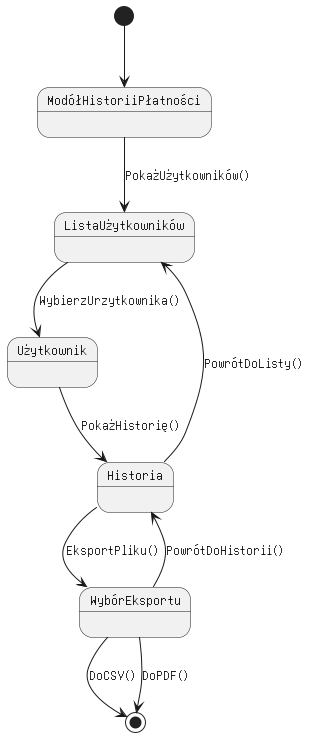
\includegraphics{diagrams/state/historia_płatności}}

\begin{enumerate}
\setcounter{enumi}{24}
\tightlist
\item
  {Przejrzyj historię płatności użytkownika}
\end{enumerate}

{Aktorzy biorący udział: Administrator}

{Cel przypadku: Przejrzenie historii płatności konkretnego użytkownika}

{Warunki początkowe: Administrator jest zalogowany do systemu i ma
uprawnienia do przeglądania historii płatności użytkowników.}

{Warunki końcowe: Administrator ma dostęp do szczegółowej historii
płatności użytkownika.}

{Główny ciąg zdarzeń:}

\begin{enumerate}
\tightlist
\item
  {Administrator wybiera opcję "Historia płatności" w panelu
  administratora.}
\item
  {System wyświetla listę użytkowników, którzy dokonali płatności.}
\item
  {Administrator wybiera użytkownika, którego historię płatności chce
  przeglądać.}
\item
  {System wyświetla szczegółową historię płatności wybranego
  użytkownika, w tym daty, kwoty oraz rodzaj płatności.}
\item
  {Administrator może przeglądać historię płatności użytkownika, a także
  eksportować ją do pliku CSV lub PDF.}
\item
  {Po zakończeniu przeglądania historii płatności, administrator może
  wrócić do panelu administratora lub wylogować się z systemu.}
\end{enumerate}

{Alternatywne ciągi zdarzeń:}

\begin{itemize}
\tightlist
\item
  {Jeśli nie ma żadnych użytkowników z dokonanymi płatnościami, system
  wyświetla komunikat, że nie ma historii płatności do wyświetlenia.}
\item
  {Jeśli nie można znaleźć użytkownika, administrator otrzymuje
  komunikat, że nie ma użytkownika o podanym adresie e-mail lub
  loginie.}
\end{itemize}

{}

{}

\begin{enumerate}
\setcounter{enumi}{25}
\tightlist
\item
  {Dodaj budynek siłowni}
\end{enumerate}

{Aktorzy biorący udział: Administrator}

{Cel przypadku: Dodanie nowego budynku siłowni do systemu zarządzania
siłownią}

{Warunki początkowe: Administrator zalogowany do systemu, posiadający
uprawnienia do dodawania nowych budynków siłowni}

{Warunki końcowe: Nowy budynek siłowni został dodany do systemu i jest
dostępny dla użytkowników}

{Główny ciąg zdarzeń:}

\begin{enumerate}
\tightlist
\item
  {Administrator wybiera opcję "Dodaj budynek siłowni"}
\item
  {System wyświetla formularz dodawania nowego budynku siłowni}
\item
  {Administrator wprowadza nazwę budynku, adres, numer telefonu i adres
  e-mail}
\item
  {Administrator wybiera zdjęcie budynku z dysku lub podaje adres URL}
\item
  {Administrator zatwierdza dodanie nowego budynku siłowni}
\item
  {System dodaje nowy budynek siłowni do bazy danych}
\item
  {System wyświetla komunikat potwierdzający dodanie nowego budynku
  siłowni}
\end{enumerate}

{Alternatywne ciągi zdarzeń:}

\begin{itemize}
\tightlist
\item
  {W przypadku błędnie wprowadzonych danych, system wyświetla komunikat
  o błędach i prosi o ich poprawienie.}
\item
  {Administrator może zrezygnować z dodania nowego budynku siłowni,
  klikając opcję "Anuluj". W takim przypadku system nie dodaje nowego
  budynku i zamyka formularz.}
\end{itemize}

{}

{}

\begin{enumerate}
\setcounter{enumi}{26}
\tightlist
\item
  {Dodaj właściciela siłowni}
\end{enumerate}

{Aktorzy biorący udział: Administrator}

{Cel przypadku: Dodanie nowego właściciela siłowni do systemu}

{Warunki początkowe: Administrator zalogowany do systemu}

{Warunki końcowe: Nowy właściciel siłowni dodany do systemu}

{Główny ciąg zdarzeń:}

\begin{enumerate}
\tightlist
\item
  {Administrator wybiera opcję "Dodaj właściciela siłowni" z panelu
  administracyjnego.}
\item
  {System wyświetla formularz dodawania nowego właściciela siłowni z
  polami takimi jak imię, nazwisko, adres e-mail, numer telefonu itp.}
\item
  {Administrator wprowadza dane nowego właściciela siłowni i zatwierdza
  formularz.}
\item
  {System przeprowadza walidację danych i dodaje nowego właściciela
  siłowni do bazy danych.}
\item
  {System wyświetla komunikat potwierdzający dodanie nowego właściciela
  siłowni.}
\end{enumerate}

{Alternatywne ciągi zdarzeń:}

\begin{itemize}
\tightlist
\item
  {W przypadku nieprawidłowych lub niekompletnych danych, system
  wyświetla informacje o błędach i prosi o wprowadzenie poprawnych
  danych.}
\item
  {Jeśli dany właściciel siłowni już istnieje w systemie, system
  informuje o tym i prosi o wprowadzenie innych danych.}
\end{itemize}

{}

{}

\begin{enumerate}
\setcounter{enumi}{27}
\tightlist
\item
  {Usuń budynek siłowni}
\end{enumerate}

{Aktorzy biorący udział: Administrator}

{Cel przypadku: Usunięcie budynku siłowni z systemu}

{Warunki początkowe: Administrator musi być zalogowany do systemu}

{Warunki końcowe: Budynek siłowni jest usunięty z systemu}

{Główny ciąg zdarzeń:}

\begin{enumerate}
\tightlist
\item
  {Administrator loguje się do systemu}
\item
  {Administrator wybiera moduł zarządzania budynkami siłowni}
\item
  {Administrator wyszukuje budynek siłowni, który chce usunąć}
\item
  {Administrator wybiera opcję usunięcia budynku siłowni}
\item
  {System wyświetla ostrzeżenie, że usunięcie budynku siłowni spowoduje
  usunięcie wszystkich informacji z nim związanych}
\item
  {Administrator potwierdza chęć usunięcia budynku siłowni}
\item
  {System usuwa budynek siłowni z systemu}
\item
  {System wyświetla informację o sukcesie operacji}
\end{enumerate}

{Alternatywne ciągi zdarzeń:}

\begin{itemize}
\tightlist
\item
  {Jeśli administrator nie może znaleźć budynku siłowni na liście, to
  system wyświetla komunikat informujący o tym fakcie. }
\item
  {W kroku 6, jeśli administrator anuluje operację usuwania budynku
  siłowni, to system wyświetla informację o anulowaniu operacji.}
\end{itemize}

{}

{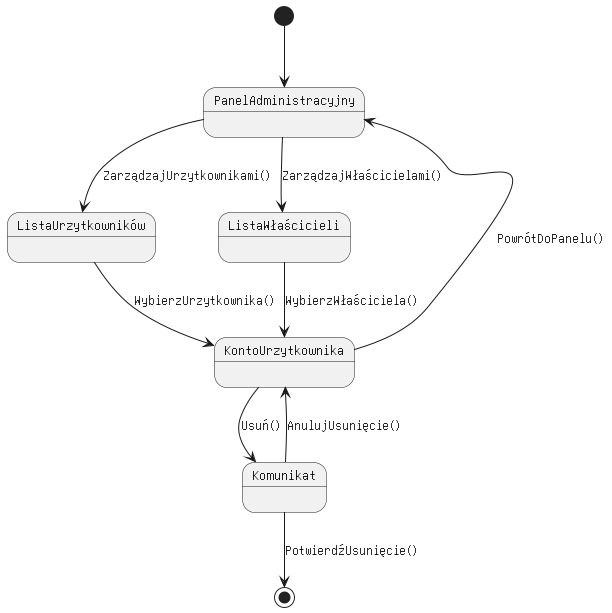
\includegraphics{diagrams/state/usuń_użytkownika.png}}

\begin{enumerate}
\setcounter{enumi}{28}
\tightlist
\item
  {Usuń użytkownika}
\end{enumerate}

{Aktorzy biorący udział: Administrator}

{Cel przypadku: Usunięcie konta użytkownika z systemu}

{Warunki początkowe: Administrator zalogowany do systemu, istnieje konto
użytkownika, które ma zostać usunięte}

{Warunki końcowe: Konto użytkownika zostaje usunięte z systemu}

{Główny ciąg zdarzeń:}

\begin{enumerate}
\tightlist
\item
  {Administrator loguje się do systemu}
\item
  {Administrator otwiera panel administracyjny i wybiera opcję "Usuń
  użytkownika"}
\item
  {System wyświetla listę wszystkich użytkowników}
\item
  {Administrator wybiera użytkownika, którego konto ma zostać usunięte}
\item
  {System wyświetla komunikat potwierdzający, że użytkownik zostanie
  usunięty z systemu wraz ze wszystkimi jego danymi}
\item
  {Administrator potwierdza usunięcie użytkownika}
\item
  {System usuwa konto użytkownika z systemu i wyświetla komunikat
  potwierdzający}
\end{enumerate}

{Alternatywne ciągi zdarzeń:}

\begin{itemize}
\tightlist
\item
  {W kroku 4 administrator nie może znaleźć użytkownika, którego konto
  ma zostać usunięte - w takim przypadku może wykonać ponowne
  wyszukiwanie lub zakończyć działanie bez usuwania konta użytkownika}
\item
  {W kroku 6 administrator może zrezygnować z usunięcia konta
  użytkownika i zakończyć działanie}
\end{itemize}

{}

{}

{}

\begin{enumerate}
\setcounter{enumi}{29}
\tightlist
\item
  {Usuń właściciela siłowni}
\end{enumerate}

{Aktorzy biorący udział: Administrator}

{Cel przypadku: Usunięcie właściciela siłowni z systemu}

{Warunki początkowe: Administrator jest zalogowany do systemu,
właściciel siłowni posiada aktywne konto w systemie}

{Warunki końcowe: Właściciel siłowni zostaje usunięty z systemu, a
wszystkie informacje związane z jego kontem są usuwane.}

{Główny ciąg zdarzeń:}

\begin{enumerate}
\tightlist
\item
  {Administrator loguje się do systemu.}
\item
  {Administrator przechodzi do modułu zarządzania użytkownikami.}
\item
  {Administrator wyszukuje konto właściciela siłowni.}
\item
  {Administrator wybiera opcję usunięcia konta właściciela siłowni.}
\item
  {System wyświetla potwierdzenie usunięcia konta.}
\item
  {Administrator potwierdza usunięcie konta.}
\item
  {System usuwa konto właściciela siłowni i wszystkie powiązane z nim
  informacje.}
\end{enumerate}

{Alternatywne ciągi zdarzeń:}

\begin{itemize}
\tightlist
\item
  {Jeśli istnieją powiązane z kontem właściciela siłowni informacje,
  system wyświetla ostrzeżenie o konieczności usunięcia tych informacji
  przed usunięciem konta. Administrator musi usunąć te informacje przed
  kontynuowaniem procedury usuwania konta.}
\item
  {Jeśli właściciel siłowni jest przypisany do jakiegoś konkretnego
  budynku, system może wyświetlić ostrzeżenie, że usunięcie właściciela
  może wpłynąć na funkcjonowanie siłowni i poprosić o potwierdzenie
  przed kontynuowaniem.}
\item
  {W kroku 3 administrator nie może znaleźć właściciela siłowni, którego
  konto ma zostać usunięte - w takim przypadku może wykonać ponowne
  wyszukiwanie lub zakończyć działanie bez usuwania konta właściciela
  siłowni.}
\item
  {W kroku 6 administrator może zrezygnować z usunięcia konta
  właściciela siłowni i zakończyć działanie.}
\end{itemize}